\documentclass[11pt]{book}

\usepackage[top=1.25in,bottom=1.25in,right=1in,left=1in]{geometry}
\usepackage[colorlinks=true, urlcolor=blue, linkcolor=violet ]{hyperref}
\usepackage{graphicx}
\usepackage{caption}
\usepackage{listings}
\usepackage{pgfplots}
\usetikzlibrary{calc,angles,quotes}
\usepackage{tikz}
\usepackage{booktabs}
\usepackage[titletoc]{appendix} 
\usepackage{xepersian}
\usepackage{lmodern} 
\usepackage{amsmath}
\usepackage{amssymb}
\usepackage{fancyhdr}

\lstset{basicstyle=\ttfamily\small}

\settextfont[Scale=1.1]{XB Niloofar}
\setlatintextfont[Scale=1.0]{Times New Roman}
\setdigitfont[Scale=1.1]{XB Niloofar}

\newcommand{\len}[1]{\lr{#1}}

\title{پاسخنامه الکترومغناطیس ریتس و میلفورد + تحلیل محاسباتی}
\author{S.Mustafa}
\date{}

\counterwithin{equation}{section}
\counterwithin{figure}{section}
\counterwithin{footnote}{section}

\begin{document}

\maketitle
\newpage

\tableofcontents

\newpage

\section{فصل اول: آنالیز برداری}

\section{فصل دوم: الکترواستاتیک}


۱.

\begin{figure}[h!]
\centering
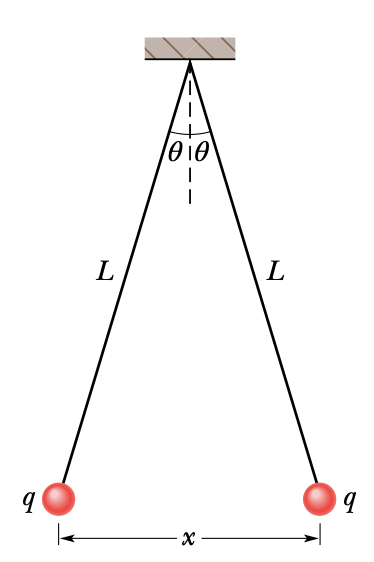
\includegraphics[width=0.2\textwidth]{2.1}
\end{figure}


۲.

\section{فصل سوم: حل‌المسائل الکترواستاتیک}

\section{فصل چهارم: میدان الکترواستاتیک در محیط‌های دی‌الکتریک}

\end{document}